%% LyX 2.4.4 created this file.  For more info, see https://www.lyx.org/.
%% Do not edit unless you really know what you are doing.
\documentclass[english]{article}
\usepackage[T1]{fontenc}
\usepackage[latin9]{inputenc}
\usepackage{units}
\usepackage{enumitem}
\usepackage{amsmath}
\usepackage{amsthm}
\usepackage{cancel}
\usepackage{geometry}
\geometry{verbose,tmargin=1in,bmargin=1in,lmargin=1in,rmargin=1in}

\makeatletter
%%%%%%%%%%%%%%%%%%%%%%%%%%%%%% Textclass specific LaTeX commands.
\numberwithin{equation}{section}
\numberwithin{figure}{section}
\newlength{\lyxlabelwidth}      % auxiliary length 

%%%%%%%%%%%%%%%%%%%%%%%%%%%%%% User specified LaTeX commands.
\usepackage{fancyhdr}
\usepackage{lastpage}
\pagestyle{fancy}
\usepackage{enumitem}
\usepackage{ifthen}
%sets math fonts to be more readable
\everymath=\expandafter{\the\everymath\displaystyle}
%\DeclareMathSizes{10}{10}{10}{10}
\usepackage{multicol}

\usepackage{tikz}
\usetikzlibrary{plotmarks}
\usepackage{pgfplots}
\pgfplotsset{compat=newest}

\usepackage{calc}
\usepackage[nomessages]{fp}

\usepackage{advdate}    % Advancing/saving dates
\usepackage{datetime}   % Dates formatting
\usepackage{datenumber} % Counters for dates
% Added by lyx2lyx
\setlength{\parskip}{\smallskipamount}
\setlength{\parindent}{0pt}

\makeatother

\usepackage{babel}
\begin{document}
\renewcommand{\author}{Dr.\,James Ashe}

\newcommand{\classNum}{131}

\newcommand{\classSec}{B}

\newcommand{\nameType}{Name:}

\newcommand{\examType}{Exam 1}

\renewcommand{\date}{\formatdate{13}{9}{2013}}

%%First page's header%%%%%%%%%%%%%%%%%%%%%%
\fancypagestyle{firststyle} %%header settings for first pagr
{
	\fancyhead[L]{MTH \classNum{}(\classSec{}) \author{}\\
	\textbf{\examType{}} \date{}}
	\fancyhead[C]{\textbf{\nameType}}
	\setlength{\headsep}{14pt}
}
%%%%%%%%%%%%%%%%%%%%%%%%%%%%%%%%%%%%%%%%%%

%%Next page's header%%%%%%%%%%%%%%%%%%%%%%%
\setlist{nolistsep}
\lhead{\classNum{}(\classSec{})} 
\chead{\textbf{\nameType}} 
\cfoot{\thepage{}~of~\pageref{LastPage}} 
\setlength{\headsep}{5pt} 
%%%%%%%%%%%%%%%%%%%%%%%%%%%%%%%%%%%%%%%%%%%

%%Various settings; see the preamble for other settings%%%%%
%%\setenumerate[0]{leftmargin=12pt,itemindent=0pt,labelwidth=0pt}
\renewcommand{\labelenumi}{\textbf{\arabic{enumi}.}}
\renewcommand{\labelenumii}{\textbf{\alph{enumii}.}}
\thispagestyle{firststyle}
%%%%%%%%%%%%%%%%%%%%%%%%%%%%%%%%%%%%%%%%%%
\newcommand{\xmax}{10}
\newcommand{\xmin}{-10}
\newcommand{\xstep}{0} %must be xmin+n
\newcommand{\ymax}{10}
\newcommand{\ymin}{-10}
\newcommand{\ystep}{0} %must be ymin+n

\newcommand{\xspace}{\vspace{1cm}}\textbf{You must show your work to receive credit.}
\begin{enumerate}
\item Use the graph to complete the following problems.\begin{multicols}{2}

\begin{enumerate}
\item {[}3 pts{]} Graph and label the point $\left(-7.5,4\right)$.\vfill
\item {[}3 pts{]} Determine the Cartesian coordinates of the point \textbf{(b)
}on the graph.

\begin{enumerate}
\item []$(4,-4)$
\end{enumerate}
\item Use the graph to determine the $x-$int(s) if any of $f(x)$.

\begin{enumerate}
\item []$4$, the point $(-4,0)$.
\end{enumerate}
\item Use the graph to determine the $y-$int(s) if any of $f(x)$. 

\begin{enumerate}
\item []$1$, the point $(0,1)$.
\end{enumerate}
\item []\renewcommand{\xmax}{10}
\renewcommand{\xmin}{-10}
\renewcommand{\xstep}{0} %must be xmin+n
\renewcommand{\ymax}{10}
\renewcommand{\ymin}{-10}
\renewcommand{\ystep}{0} %must be ymin+n
%%%%%%%
\begin{tikzpicture} 
\begin{axis}[height=5cm, 
	width=5cm, 
	axis lines=middle,
	minor x tick num={4},
	minor y tick num={4},
	grid=both,
	%xtick={0,50,...,250},
	%ytick={0,10,20,...,40},
	%axis line style={-latex}, 
	xmin=\xmin,xmax=\xmax, 
	ymin=\ymin,ymax=\ymax,
	%restrict y to domain=-1:10,
	%no markers, 
	xlabel={$x$},ylabel={$y$}, 
	%every axis x label/.append style={anchor=north}, 
	%every axis y label/.append style={anchor=east}
	]
	
	\addplot[color=black,solid,mark=*] coordinates {(0,1)} node[right] {\footnotesize{$(0,1)$}};
	\addplot[color=black,solid,mark=*] coordinates {(-4,0)} node[above left] {\footnotesize{$(-4,0)$}};
	\addplot[color=blue,solid,mark=*] coordinates {(-7.5,4)} node[above] {\textbf{(a)}};
	\addplot[color=black,solid,thick,mark=*] coordinates {(4,-4)} node[right] {$\textbf{(b)}$};
	\addplot[domain=\xmin:\xmax,thick,samples=100,draw=red,<->]{1/2*(x^2+1/2)*(x+4)} node[pos=.65,above] {$f(x)$};
	
\end{axis}
\end{tikzpicture}
\end{enumerate}
\end{multicols}
\end{enumerate}
\emph{Solve the linear equations. }
\begin{enumerate}[resume]
\item $2x+10=4$
\begin{eqnarray*}
2x & = & -6\\
x & = & -3
\end{eqnarray*}
\vfill
\item $3(x-1)+13=-(x+5)$
\begin{eqnarray*}
3x-3+13 & = & -x-5\\
4x & = & -15\\
x & = & \nicefrac{-15}{4}
\end{eqnarray*}
\vfill
\item $9x-(3+9x)=9$
\begin{eqnarray*}
9x-3-9x & = & 9\\
-3 & \neq & 9\Rightarrow\mbox{No Solution}
\end{eqnarray*}
\vfill
\item $\frac{3x}{2}-x=\frac{x}{10}-\frac{8}{5}$
\begin{eqnarray*}
10\left(\frac{3x}{2}-x\right) & = & \left(\frac{x}{10}-\frac{8}{5}\right)10\\
15x-10x & = & x-16\\
4x & = & -16\\
x & = & -4
\end{eqnarray*}
\vfill
\item $\frac{x+5}{3}=\frac{5}{3}+\frac{x-8}{2}$
\begin{eqnarray*}
6\left(\frac{x+5}{3}\right) & = & 6\left(\frac{5}{3}+\frac{x-8}{2}\right)\\
2\left(x+5\right) & = & 10+3(x-8)\\
2x+10 & = & 10+3x-24\\
-x & = & -24\Rightarrow x=24
\end{eqnarray*}
\vfill\newpage
\end{enumerate}
\emph{Identify any restrictions on the variable, and solve the rational
equation. }
\begin{enumerate}[resume]
\item $\frac{2}{3}=\frac{4}{x}+1$
\[
x\neq0
\]
 
\begin{eqnarray*}
3x\left(\frac{2}{3}\right) & = & 3x\left(\frac{4}{x}+1\right)\\
2x & = & 12+3x\\
-12 & = & x\Rightarrow x=-12
\end{eqnarray*}
\vfill
\end{enumerate}
\emph{Solve the quadratic equations by factoring.}
\begin{enumerate}[resume]
\item $x^{2}-2x=8$.
\begin{eqnarray*}
x^{2}-2x-8 & = & 0\\
(x-4)(x+2) & = & 0\\
 & \Rightarrow & x=4\mbox{ and }x=-2
\end{eqnarray*}
\vfill
\item $4x^{2}-8x-32=0$.
\begin{eqnarray*}
4(x^{2}-2-8) & = & 0\\
4(x-4)(x+2) & = & 0\\
 & \Rightarrow & x=4\mbox{ and }x=-2
\end{eqnarray*}
\vfill
\end{enumerate}
\emph{Solve the quadratic equation using the square root property.}
\begin{enumerate}[resume]
\item $(x-3)^{2}-5=7$
\begin{eqnarray*}
(x-3)^{2} & = & 12\\
\sqrt{(x-3)^{2}} & = & \pm\sqrt{12}\\
x-3 & = & \pm\sqrt{4}\sqrt{3}\\
x & = & 3\pm2\sqrt{3}
\end{eqnarray*}
\vfill
\end{enumerate}
\emph{Solve the quadratic.}
\begin{enumerate}[resume]
\item $x^{2}+2x=13$.

\begin{enumerate}[resume]
\item []By completing the square. $b=2\Rightarrow\left(\frac{2}{2}\right)^{2}=1$
\begin{eqnarray*}
x^{2}+2x+1 & = & 13+1\\
(x+1)^{2} & = & 14\\
x+1 & = & \pm\sqrt{14}\\
x & = & -1\pm\sqrt{14}
\end{eqnarray*}
\item []Using the quadratic formula; $x^{2}+2x-13=0$; $a=1,\,b=2,\,\mbox{and }c=-13$.
\begin{eqnarray*}
x & = & \frac{-(2)\pm\sqrt{(2)^{2}-4(1)(-13)}}{2(1)}\\
 & = & \frac{-2\pm\sqrt{56}}{2}=\frac{-2\pm2\sqrt{14}}{2}\\
 & = & -1\pm\sqrt{14}
\end{eqnarray*}
\vfill
\end{enumerate}
\end{enumerate}
\newpage\emph{Solve the problems}
\begin{enumerate}[resume]
\item {[}7 pts{]} When three times a number is subtracted from eight times
the same number the result is 20. What is the number?

\begin{enumerate}[resume]
\item []
\begin{eqnarray*}
8x-3x & = & 20\\
5x & = & 20\\
x & = & 4
\end{eqnarray*}
\vfill
\end{enumerate}
\item {[}7 pts{]} John buys house for \$100,000. If the house increases
in value by \$3500 per year. How long until it doubles in value (i.e.,
how long until it is worth \$200,000)?

\begin{enumerate}[resume]
\item []
\begin{eqnarray*}
100,000+3500x & = & 200,000\\
3500x & = & 100,000\\
x & \approx & 28.57\mbox{ years}
\end{eqnarray*}
\vfill
\end{enumerate}
\item {[}Bonus{]} Jane is playing playing receiver on a flag football team.
She runs $10$ yards straight down-field, makes a $90^{\circ}$turn
to her right, and runs another $5$ yards straight towards the sideline.
How far is she from her original position.

\begin{enumerate}[resume]
\item []The distance is the hypotenuse of a right triangle. \begin{multicols}{2}\hfill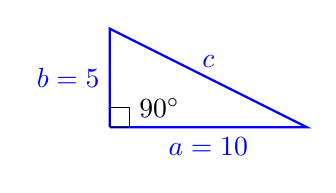
\begin{tikzpicture} [scale=.25]
	\draw [blue,thick] (0,0)--(10,0) node[midway,below] {$a=10$} --(0,5) node[midway,above] {$c$} --(0,0) node[midway,left] {$b=5$} ;
	\draw [black] (0,0)--(1,0)--(1,1) node[above,right] {$90^{\circ}$} --(0,1)--(0,0);
\end{tikzpicture}\columnbreak
\item []Use Pythagoras' theorem to solve for $c$, 
\begin{eqnarray*}
c^{2} & = & 10^{2}+5^{2}\\
c & = & \sqrt{125}\mbox{ yards}
\end{eqnarray*}
\end{multicols}\vfill
\end{enumerate}
\end{enumerate}

\end{document}
